\begin{document}
\graphicspath{ {images/slt/} }

\section{Structure Learning -- Trees}

\subsection{Structure Learning for an Undirected Tree-Structured Graphical Model: The Chow-Liu Algorithm}

At this point we've covered parameter learning for undirected trees, where we assume we know the tree structure. But what if we don't know what tree to even use? We now look at an algorithm called the Chow-Liu algorithm that learns which tree to use from training data, again using maximum likelihood. Once more, information measures appear, where mutual information plays a pivotal role. Recall that mutual information tells us how far two random variables are from being independent. A key idea here is that to determine whether an edge between two random variables should be present in a graphical model, we can look at mutual information.

The idea is that we have random variables $X_1$ up through $X_k$. These you can think of as nodes in a undirected graphical model. But we don't know which edges should be in this graphical model. And restricting ourself to trees, the question is, which tree should we use? To help us answer this question, we're going to have access to training data. We see $n$ i.i.d. samples from this graphical model, where for each of the samples, of course, we see everything, $x_1^{(i)},\dots ,x_k^{(i)}$. So this is the $i$-th training data point and $i = 1 \dots n$. Just as a comment, the number of possible trees here is humongous, actually $k^{k-2}$. This from a result called Cayley's formula, which grows even faster than exponential, it's super exponential. Somehow, we're going to search this huge space of possible trees to select the best tree. It turns out, doing that can be done very quickly. To select the tree we're going to use maximum likelihood. We're going to pick the tree $T$ here. 

{\centering$\displaystyle \widehat{T}=\arg\max_{T} \bigg\{\max_{\theta_T} \log \prod_{i=1}^n p_{x_1 \dots x_k}^{(x_1^{(i)},\dots ,x_k^{(i)}; T, \theta_T)} \bigg\}$ \par}

In this case, we know that there are $k$ nodes, but where are the edges? You can think of $T$ as just specifying which edges are present that result in a tree across $k$ nodes, with $k-1$ edges. So we're trying to find the best tree such that once we fix a tree, then we can do maximum likelihood for that specific tree $T$. 

To solve this optimization problem, it turns out there's a very clean algorithm. To get to it, we're going to simplify what's in the curly braces:

\begin{eqnarray*}
\text{For specific tree } T: \\
& & \max_{\theta_T} \log \prod_{i=1}^n p_{x_1 \dots x_k}^{(x_1^{(i)},\dots ,x_k^{(i)}; T, \theta_T)}  \\&=& \log \prod_{i=1}^n \bigg[ \widehat{p}(x_r^{(i)}) \prod_{j \ne r} \widehat{p}(x_r^{(i)} | x_{\pi(j)}^{(i)}) \bigg] \\
&=& \sum_{i=1}^n \log \widehat{p}(x_r^{(i)}) + \sum_{j \ne r} \sum_{i=1}^n \log \widehat{p}(x_r^{(i)} | x_{\pi(j)}^{(i)}) \\
\end{eqnarray*}

We have the log likelihood across the training data. Here, we're parameterizing by both what the tree is and then, once we know the tree, some set of parameters $\theta_T$ for the tree. We can arbitrarily choose a root $r$ and drop the subscripts just to save some writing. So the factorization is $p(x_r^{(i)})$ times the product from all the nodes that are not equal to the root $p(x_r^{(i)} | x_{\pi(j)}^{(i)})$. We want to take the maximum over all the $\theta_T$'s, meaning we want to plug in the best possible values of the parameters into this expression. But we know from the parameter learning video that the best choice of $\theta$ is going to correspond to the empirical distributions. All we need to do is replace the probability distributions $p$ with the empirical versions $\widehat{p}$, which give us the desired max. As a reminder, $\widehat{p}(x_r^{(i)})$ is the empirical distribution of random variable $X_r$. Evaluated at some value $a$ this is just equal to the fraction of times $a$ appears in the training data. So $\widehat{p}(x_r^{(i)}) = \frac{1}{n} \sum_{i=1}^n \mathbf{1} \{x_r^{(i)}=a\}$. This is just an example of how you get these empirical distributions. The empirical conditional probability table, as a reminder, is going to be the fraction of times we see that these two random variables in our training data jointly take on two specific values divided by the number of times we see this random variable taking on a specific value in our training data. That's what these $\widehat{p}$'s are. 

\begin{eqnarray*}
& & \sum_{i=1}^n \log \widehat{p}(x_r^{(i)}) + \sum_{j \ne r} \sum_{i=1}^n \log \widehat{p}(x_r^{(i)} | x_{\pi(j)}^{(i)}) \\
&=& \sum_a \bigg[ \sum_{i=1}^n \mathbf{1} \{ x_r^{(i)} = a\} \bigg] \log \widehat{p}_{x_r} (a) + \sum_{j \ne r} \sum_{a,b} \bigg[ \sum_{i=1}^n \mathbf{1} \{ x_j^{(i)} = a, x_{\pi(j)}^{(i)} = b \} \bigg] \log \widehat{p}_{x_j | x_{\pi(j)}} (a|b) 
\end{eqnarray*}

Next we introduce a different summation to split up what the possible values of this random variable are. We were doing this for the conditional distributions earlier. But now, we're going to do it for all of them, counting up how many times we see each particular value. %You can use the definition of conditional probability even for an empirical distribution, because an empirical distribution is still a distribution. So we can write this piece as p hat of X j, X pi j of a comma b divided by-- and then since we're conditioning on X pi j, it's going to be p hat of X pi j evaluated at b. So we're going to have this. A

\begin{eqnarray*}
& & \sum_a \underbrace{\bigg[ \sum_{i=1}^n \mathbf{1} \{ x_r^{(i)} = a\} \bigg] \log \widehat{p}_{x_r} (a)}_{n p_{x_r} (a)} + \sum_{j \ne r} \sum_{a,b} \underbrace{\bigg[ \sum_{i=1}^n \mathbf{1} \{ x_j^{(i)} = a, x_{\pi(j)}^{(i)} = b \} \bigg]}_{n \widehat{p}_{x_j, x_{\pi(j)}} (a,b) } \log \widehat{p}_{x_j | x_{\pi(j)}} (a|b) \\
&=& n \bigg[ \underbrace{\sum_a p_{x_r} (a) \log \widehat{p}_{x_r} (a)}_{-H(\widehat{p}_{x_r})} + \underbrace{\sum_{j \ne r} \sum_{a,b} \widehat{p}_{x_j, x_{\pi(j)}} (a,b) \log \frac{ \widehat{p}_{x_j, x_{\pi(j)}} (a,b) }{ \widehat{p}_{x_{\pi(j)}} (b) \widehat{p}_{x_j}(a)} }_{\sum_{j \ne r} D(\widehat{p}_{x_j, x_{\pi(j)}})} \widehat{p}_{x_j}(a) \bigg] \\
&=& n \bigg[ -H(\widehat{p}_{x_r}) + \sum_{j \ne r} \underbrace{D(\widehat{p}_{x_j, x_{\pi(j)}})}_{\widehat{I}(x_j, x_{\pi(j))}} + \underbrace{\sum_a \widehat{p}_{x_j}(a) \log \widehat{p}_{x_j}(a)}_{-H(\widehat{p}_{x_j}} \bigg] \\
&=& n \bigg[ -\sum_{j \in V} H(\widehat{p}_{x_j}) + \sum_{(i,j) \in E} \widehat{I}(x_i;x_j) \bigg]
\end{eqnarray*}

The first term is related to the negative entropy. The log is natural log, but that's OK. We can still talk about the entropy, it's just in terms of ``nats'' not bits. The second term we multiply top and bottom by $\widehat{p}_{x_j}(a)$, which is just multiplying by 1. That gives us a term which is the information divergence $D(\widehat{p}_{x_j, x_{\pi(j)}})$. The basic idea is we're looking at how far the empirical joint distribution is from a product of two empirical marginal distributions. You can think of this as saying, how far is this empirical joint distribution from being independent. This is called the mutual information between these two random variables. But it's not actually these two random variables, it's the empirical versions of them. So we'll denote this as the empirical mutual information between $x_j$ and $x_{\pi(j))}$. Again, the mutual information would be this exact same thing except with the true distributions, rather than the empirical distributions. Now, when we're looking at the empirical distributions, we just get this empirical mutual information instead. So that accounts for one piece of the second term. We have another piece, and this will become a minus entropy of the empirical distribution of $X_j$. Once we put all these pieces together, there is a minus entropy of the root node and a minus entropy for all the other nodes. So we're going to have a sum over all the nodes $V$ of minus entropy of the empirical distribution of $X_j$. We're also going to have the empirical mutual information $\widehat{I}(x_i;x_j)$ for $(i, j)$ within the edges in the tree.

The bottom line is this is equal to the maximum likelihood across parameters for a specific tree $T$. Note that to choose the best possible tree, the nodes aren't going to change, so the negative entropy term is going to be the same across any tree. The only thing that changes is the mutual information term that depends on the edges in the tree. So to figure out what the best tree is possible we just want to maximize this $\sum_{(i,j) \in E} \widehat{I}(x_i;x_j)$ term. 

Now we want an algorithm that maximizes this across all possible trees. The basic idea of the algorithm is to start with a graph with no edges and incrementally add edges until we get the best tree according to maximum likelihood. For the first edge we add, we're going to look at all pairs of random variables to find which one has the highest empirical mutual information, and we're going to add that edge. Then we're going to repeat that process -- we're going to find the pair of random variables with the second-highest empirical mutual information and so forth where we make sure that whenever we add an edge we don't introduce a cycle. And after we add enough edges we're going to get a tree and that's actually the best tree. This is called the Chow-Liu algorithm, illustrated with a simple four-node example. 

{\centering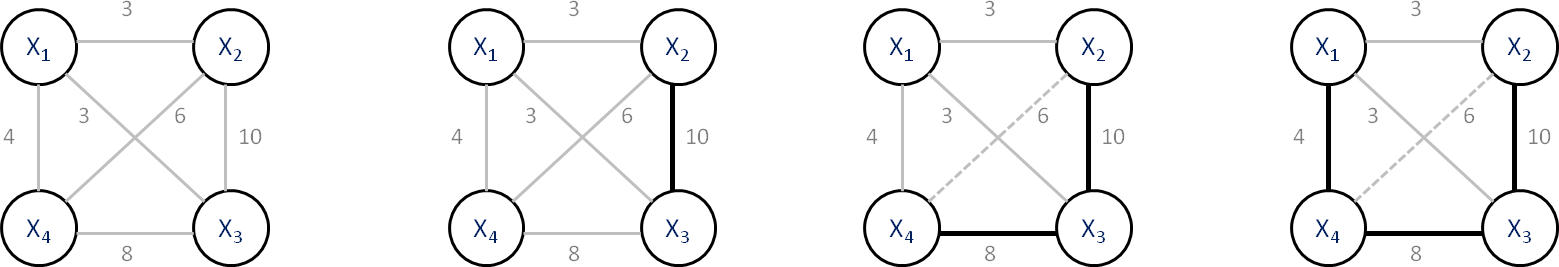
\includegraphics[scale=0.4]{Chow_Liu4a} \par}

Here we have $k=4$ for $X_1 \dots X_4$, and in gray are all the edges you could possibly have. For each of these edges we have a gray number, the empirical mutual information quantities. In practice these would be computed based on your training data. In the Chow-Liu algorithm we ask, what is the highest empirical mutual information? It's 10, so that is first edge to be added. The second highest edge is 8, which we add. Then in the next step, the third highest one is 6, but if we add this edge it will form a cycle, so skip that and move on to the next highest, which is 4, and we add that. At this point the algorithm would stop because adding anything else would form a cycle. So at this point the Chow-Liu algorithm would output a tree, denoted by the solid black lines, and that would be the maximum likelihood estimate for the best possible tree we could use. 

The general idea is very simple. We start with a graph with no edges. And then for all pairs of random variables $(i,j)$ we compute the empirical mutual information quantities $\widehat{I}(X_i; X_j)$, the gray numbers. Next we sort these empirical mutual information quantities from highest to lowest. And then starting from the highest and going all the way to the lowest we're going to add edges, except we skip adding an edge if it results in a cycle. And this algorithm will always terminate because for a graph with $k$ nodes, any tree for that graph is going to have $k-1$ edges. For example in this case, any tree for this graph has 3 edges. That is the Chow-Liu algorithm. Given training data we can learn what is the maximum likelihood estimate for the tree that best explains the data. 

\end{document}
